% 1988 年全国卷理科第 19 题：四棱锥
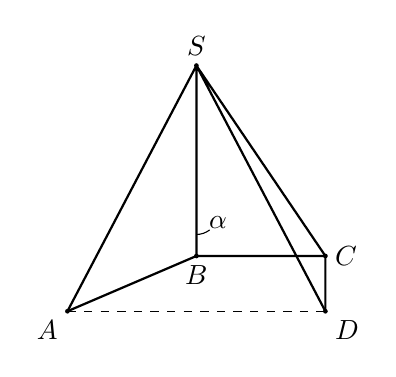
\begin{tikzpicture}[scale=0.78,>=stealth]
  \coordinate (S) at (2.1,4.0);
  \coordinate (B) at (2.1,0.9);
  \coordinate (A) at (0,0);
  \coordinate (C) at (4.2,0.9);
  \coordinate (D) at (4.2,0);
  \draw[thick] (S)--(A) (S)--(B) (S)--(C) (S)--(D);
  \draw[thick] (A)--(B)--(C)--(D);
  \draw[dashed] (A)--(D) (S)--(B);
  \draw (2.1,1.25) arc (-90:-52:0.35);
  \node at (2.45,1.45) {$\alpha$};
  \fill (S) circle (1.1pt) node[above] {$S$};
  \fill (A) circle (1.1pt) node[below left] {$A$};
  \fill (B) circle (1.1pt) node[below] {$B$};
  \fill (C) circle (1.1pt) node[right] {$C$};
  \fill (D) circle (1.1pt) node[below right] {$D$};
\end{tikzpicture}
